\documentclass[11pt,a4paper]{article}
\usepackage[utf8]{inputenc}
\usepackage[spanish]{babel}
\usepackage{amsmath}
\usepackage{graphicx}
\usepackage{geometry}
\geometry{left=2.5cm,right=2.5cm,top=2.5cm,bottom=2.5cm}

\title{Simulación y Optimización de Plantas Industriales mediante SIMUL8: Análisis Operativo y Financiero}
\author{Mateo Hidalgo, Juan Martin Funes Castro, Matteo Pratellesi, Manuel Roby y Juan Cruz Solchaga}
\date{Universidad Nacional de Cuyo}

\begin{document}
\maketitle

\begin{abstract}
Este documento técnico presenta un análisis operativo y una guía metodológica para el modelado dinámico de plantas industriales utilizando el software de simulación de eventos discretos SIMUL8[cite: 3, 92]. El objetivo principal radica en evaluar la viabilidad financiera, la eficiencia de los flujos de trabajo concurrentes y la capacidad de absorción de la planta[cite: 4, 93]. A través de la parametrización de variables de tiempo de ciclo fijas y distribuciones estocásticas, se determinó el comportamiento de los inventarios intermedios, cuellos de botella y la rentabilidad integral[cite: 5, 94]. Los resultados financieros demuestran un balance superavitario, validando la configuración de recursos implementada[cite: 6, 79].
\end{abstract}

\section{Introducción}
El diseño de sistemas en la industria automotriz moderna exige metodologías capaces de predecir el comportamiento dinámico de los procesos antes de su implementación física. Las herramientas de simulación de eventos discretos permiten representar sistemas complejos donde los cambios ocurren en momentos específicos del tiempo, facilitando la identificación precisa de ineficiencias logísticas y operacionales.

En este módulo, se empleó el software SIMUL8 para modelar de manera integral una línea de producción y comercialización de componentes automotrices. A diferencia de los análisis de capacidad estáticos tradicionales, este modelo permitió estudiar la concurrencia de flujos, la asignación dinámica de recursos humanos y tecnológicos limitados, y el impacto directo de las variaciones operacionales sobre los estados de resultados financieros integrados (Income Statement).

La simulación desarrollada abarca desde el ingreso de suministros hasta la atención final de los clientes, permitiendo evaluar la eficiencia del flujo en los procesos de ensamble, el control de calidad y la gestión de la demanda.

\section{Fundamentos del Entorno SIMUL8}
El software se fundamenta en la interacción de componentes básicos orientados a objetos que replican la dinámica de una cadena de valor[cite: 19]. Los elementos fundamentales incluyen:
\begin{itemize}
    \item \textbf{Start Centers / Entry Points:} Puntos de generación donde ingresan las materias primas o los clientes al sistema bajo una tasa de arribo específica[cite: 22].
    \item \textbf{Queues / Tolvas de Espera:} Zonas de acumulación pasiva que albergan entidades en espera de ser procesadas, absorbiendo la variabilidad de los arribos y permitiendo medir los niveles de inventario en proceso (WIP)[cite: 23, 137].
    \item \textbf{Work Centers / Puestos de Trabajo:} Unidades operativas activas donde se consume tiempo para transformar las entidades, las cuales poseen eficiencias, capacidades y costos de uso asociados[cite: 24, 25].
    \item \textbf{Exit Houses / End Points:} Puntos de salida que contabilizan el egreso
de productos terminados, ventas exitosas o pérdidas del sistema.
    \item \textbf{Resources / Operarios:} Recursos humanos o mecánicos limitados requeridos por los puestos de trabajo para ejecutar sus operaciones de forma sincronizada[cite: 27].
\end{itemize}

\section{Evolucion y Aprendizaje del Modelo}
El desarrollo del simulador no fue un proceso estático, sino que siguió una trayectoria de aprendizaje iterativo dividida en fases críticas que permitieron comprender la interacción profunda entre la ingeniería de procesos, la logística de suministro y la gestión financiera integral:

\textbf{3.1 Modelado de la Línea de Producción}
Inicialmente, el enfoque se centró exclusivamente en la lógica física del procesamiento automotriz. Se diagramó la llegada de insumos a través de transporte logístico y su posterior distribución hacia las tres estaciones de ensamble concurrentes. En esta etapa se parametrizaron los Work Centers y se asignaron tiempos de ciclo coherentes con la capacidad operativa instalada. El aprendizaje clave consistió en identificar cómo la acumulación de inventario en proceso (WIP) dentro de las colas intermedias revelaba de forma inmediata los cuellos de botella del sistema físico, permitiendo ajustar la capacidad de cada estación antes de avanzar hacia la integración de servicios.

\textbf{3.2 Integración de la Atención al Cliente y Flujos de Venta}
Una vez estabilizado el flujo de manufactura, el modelo se expandió hacia el eslabón comercial. Se incorporó una "Oficina de Ventas de Autopartes" atendida por personal dedicado, lo cual transformó el simulador de un modelo de producción pura a uno de sincronización de demanda. Esta fase fue fundamental para comprender que una alta eficiencia en los ensambles finales no genera valor real si el punto de venta actúa como un cuello de botella restrictivo o si la tasa de arribo de clientes no permite absorber el nivel de producción de la planta, evidenciando la importancia de equilibrar el push de fábrica con el pull de mercado.

\textbf{3.3 Parametrización y Optimización de Escenarios}
La etapa final consistió en la conversión de variables operativas en métricas financieras. Se introdujeron los valores de costo asociados a la logística de materiales, la tarifa horaria de la mano de obra y el retorno esperado por la venta de componentes procesados. A través de la simulación de múltiples escenarios, se observó cómo pequeñas variaciones en los tiempos de ciclo o en la gestión de las estaciones de control de calidad modifican drásticamente el balance final. Este proceso permitió transformar una configuración operativa con ineficiencias en una estructura optimizada, capaz de maximizar los resultados financieros integrados (Income Statement) de la simulación.

\section{Modelado de la Industria}
El sistema desarrollado para la producción y comercialización de vehículos integra de manera síncrona la cadena productiva con la dinámica de captación de demanda. El layout general implementado se visualiza en la imagen

\begin{center}
    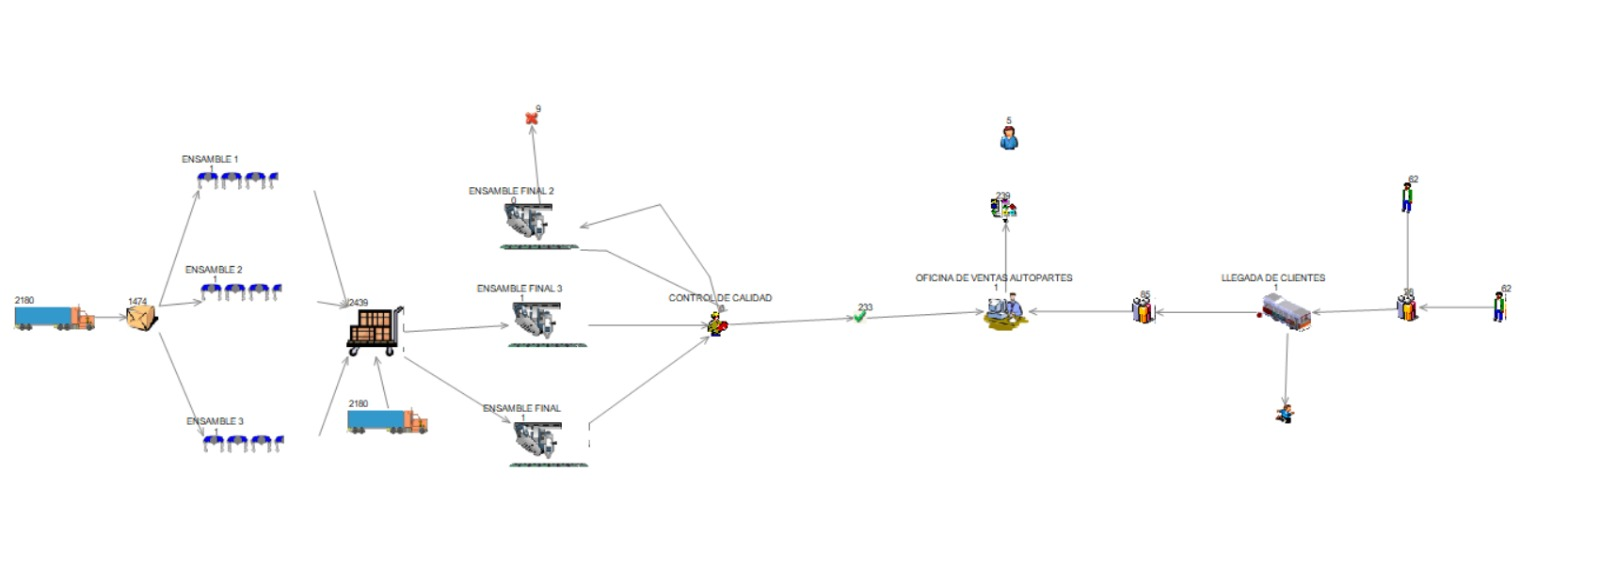
\includegraphics[width=0.5\textwidth]{simulacionimagen.jpeg}
\end{center}
\textbf{4.1 Estructura de la Rama Productiva}
La manufactura se divide en fases consecutivas de abastecimiento, ensamble y control de calidad:

\textbf{Ingreso de Materia Prima:} Representa la llegada de insumos base al sistema. Se configuró con una distribución constante (Fixed) con un valor de 11 minutos y un costo de adquisición asociado de \$400 por unidad.

\textbf{Puestos de Ensamble Concurrentes:} El sistema de entrada alimenta en paralelo a tres estaciones homogéneas denominadas Ensamble 1, Ensamble 2 y Ensamble 3. Cada puesto cuenta con restricciones estrictas de recursos (operarios asignados) y tiempos de ciclo definidos para el armado de 10 minutos.

\textbf{Control de Calidad:} Los subconjuntos convergen en una estación central de inspección. Esta etapa es crítica, ya que filtra el producto conforme antes de su paso a la fase comercial.

\textbf{4.2 Estructura de la Rama de Clientes}
Representa la llegada de la demanda al establecimiento mediante transporte corporativo:

\textbf{Fuentes de Demanda}: Se modelaron flujos de clientes independientes que arriban al sistema buscando completar la compra de vehículos.

\textbf{Logística de Espera}: Los clientes se acumulan en un área de recepción antes de ser atendidos, donde se evalúa su tolerancia a las demoras antes de abandonar las instalaciones. El 90\% de los clientes espera en su lugar,mientras el 10\% abandona las instalaciones frustrados por la demora. Cada abandono de las instalaciones recibe penalizaciones de \$1.

\textbf{4.3 Unión de Ramas: Oficina de Ventas}
Las trayectorias de los clientes y los vehículos aprobados convergen de forma síncrona en la Oficina de Ventas de Autopartes. Este nodo de acoplamiento es atendido por personal fijo y trabaja bajo una distribución de tiempo específica por transacción. Cada operación completada despacha la unidad hacia la salida del sistema, generando el ingreso bruto (Revenue) \$2000 consolidado de la empresa.
\end{itemize}

\section{Análisis de Resultados Financieros y Operacionales}

La simulación fue ejecutada bajo parámetros rigurosos de tiempo de operación, configurados en las propiedades del reloj del sistema (\textit{Clock Properties}) detallados en la Tabla 1. El periodo consolidado de análisis corresponde a una semana tipo de actividad industrial (2400 minutos).

\begin{table}[htbp]
\centering
\caption{Parámetros de temporización de la corrida de simulación.}
\begin{tabular}{ll}
\toprule
\textbf{Parámetro del Reloj} & \textbf{Valor Asignado} \\ \midrule
Unidades de Tiempo & Minutos \\
Formato de Hora & Tiempo y Día (Clock Face) \\
Días Laborales Semanales & 5 días \\
Tiempo de Jornada Diaria & 8 horas (08:00 a 16:00) \\
Período de Estabilización (\textit{Warm Up}) & 30 minutos \\
Período de Recolección de Datos & 2370 minutos \\
\textbf{Tiempo Total de Simulación por Corrida} & \textbf{2400 minutos (1 Semana)} \\ \bottomrule
\end{tabular}
\end{table}

\subsection{Evaluación del Balance de Ingresos y Costos}
El costo operativo de la mano de obra se calculó de forma exacta a partir de la tarifa corporativa de \$100/min por operario. Para la plantilla global de 12 empleados trabajando en simultáneo durante los 2400 minutos de la semana, el costo fijo de personal asciende a \$2880000. 

Al procesar la corrida en la herramienta financiera integrada de SIMUL8 (\textit{Finance Income Statement}), el sistema arrojó métricas estables que validan la rentabilidad de la configuración actual:
\begin{itemize}
    \item \textbf{Costos Totales Operativos:} $\approx \$3000000$ (incluye el costo fijo de la plantilla de personal y la adquisición de materia prima.
    \item \textbf{Ingresos Totales Brutos (\textit{Revenue}):} $\approx \$47800000$(acumulados por la venta de automotores).
    \item \textbf{\textit{Utilidad Neta Semanal}:} $\approx +\$1780000$
\end{itemize}

El resultado positivo marca que la venta de productos supera tanto el costo de la materia prima utilizada como el gasto de los sueldos de los 12 operarios que trabajan en la industria. 

\section{Conclusión}
A diferencia de los análisis de capacidad estáticos tradicionales, la simulación de eventos discretos expone la interacción real entre variables determinísticas de manufactura y arribos estocásticos de demanda. Los balances arrojados confirman que la correcta configuración de recursos humanos y líneas paralelas permite absorber los costos operativos y fijos, logrando una utilidad neta semanal y validando la sostenibilidad financiera del sistema. Esta metodología resulta crítica para justificar inversiones de capital, dimensionar inventarios y mitigar riesgos en entornos complejos.

\end{document}